\section{The Fisher matrix}\label{sec:analysis}
For each black hole metric described in Sec.\ \ref{sec:spacetimes} the Iron line and thermal spectra are characterised by a small number of parameters $\vec{\theta}$; e.g.\ for the Iron line spectra $h(\vec{\theta})$, $\vec{\theta}=(A,a,\iota,q,r_{out},\vec{\epsilon})$, where $A$ is an overall multiplicative factor relating to the unknown total luminosity and distance to the source, $a$ is the spin parameter, $\iota$ is the disk inclination, $q$ is the emissivity index described in Sec.\ \ref{subsec:line}, $r_{out}$ is the outer radius of the disk and $\vec{\epsilon}$ is the vector of any deformation parameters. Given a measured spectrum, $s$, the challenge is to infer the posterior probability density on these parameters, $P(\vec{\theta}|s,I)$. The peak of this distribution is positioned at the best estimate of $\vec{\theta}$, and the characteristic width of the peak in each parameter direction indicates the uncertainty. The posterior probability density is related to the likelihood of the data given the parameters, $P(s|\vec{\theta},I)$, via Bayes theorem,
\begin{equation}\label{eq:Bayes} P(\vec{\theta}|s)= \frac{P(s|\vec{\theta})P(\vec{\theta})}{P(s)}\; ;\end{equation}
where $P(\vec{\theta})$ is the prior probability density of the parameters and $P(s)$ is the normalisation constant known as the evidence,
\begin{equation} P(s)=\int\textrm{d}\vec{\theta}\;P(s|\vec{\theta})P(\vec{\theta}) \;.\end{equation}
For all calculations performed in this paper flat priors were assumed over all physically allowed regions of parameter space so the posterior is simply proportional to the likelihood within this region. 

\begin{figure*}[t]
 \centering
 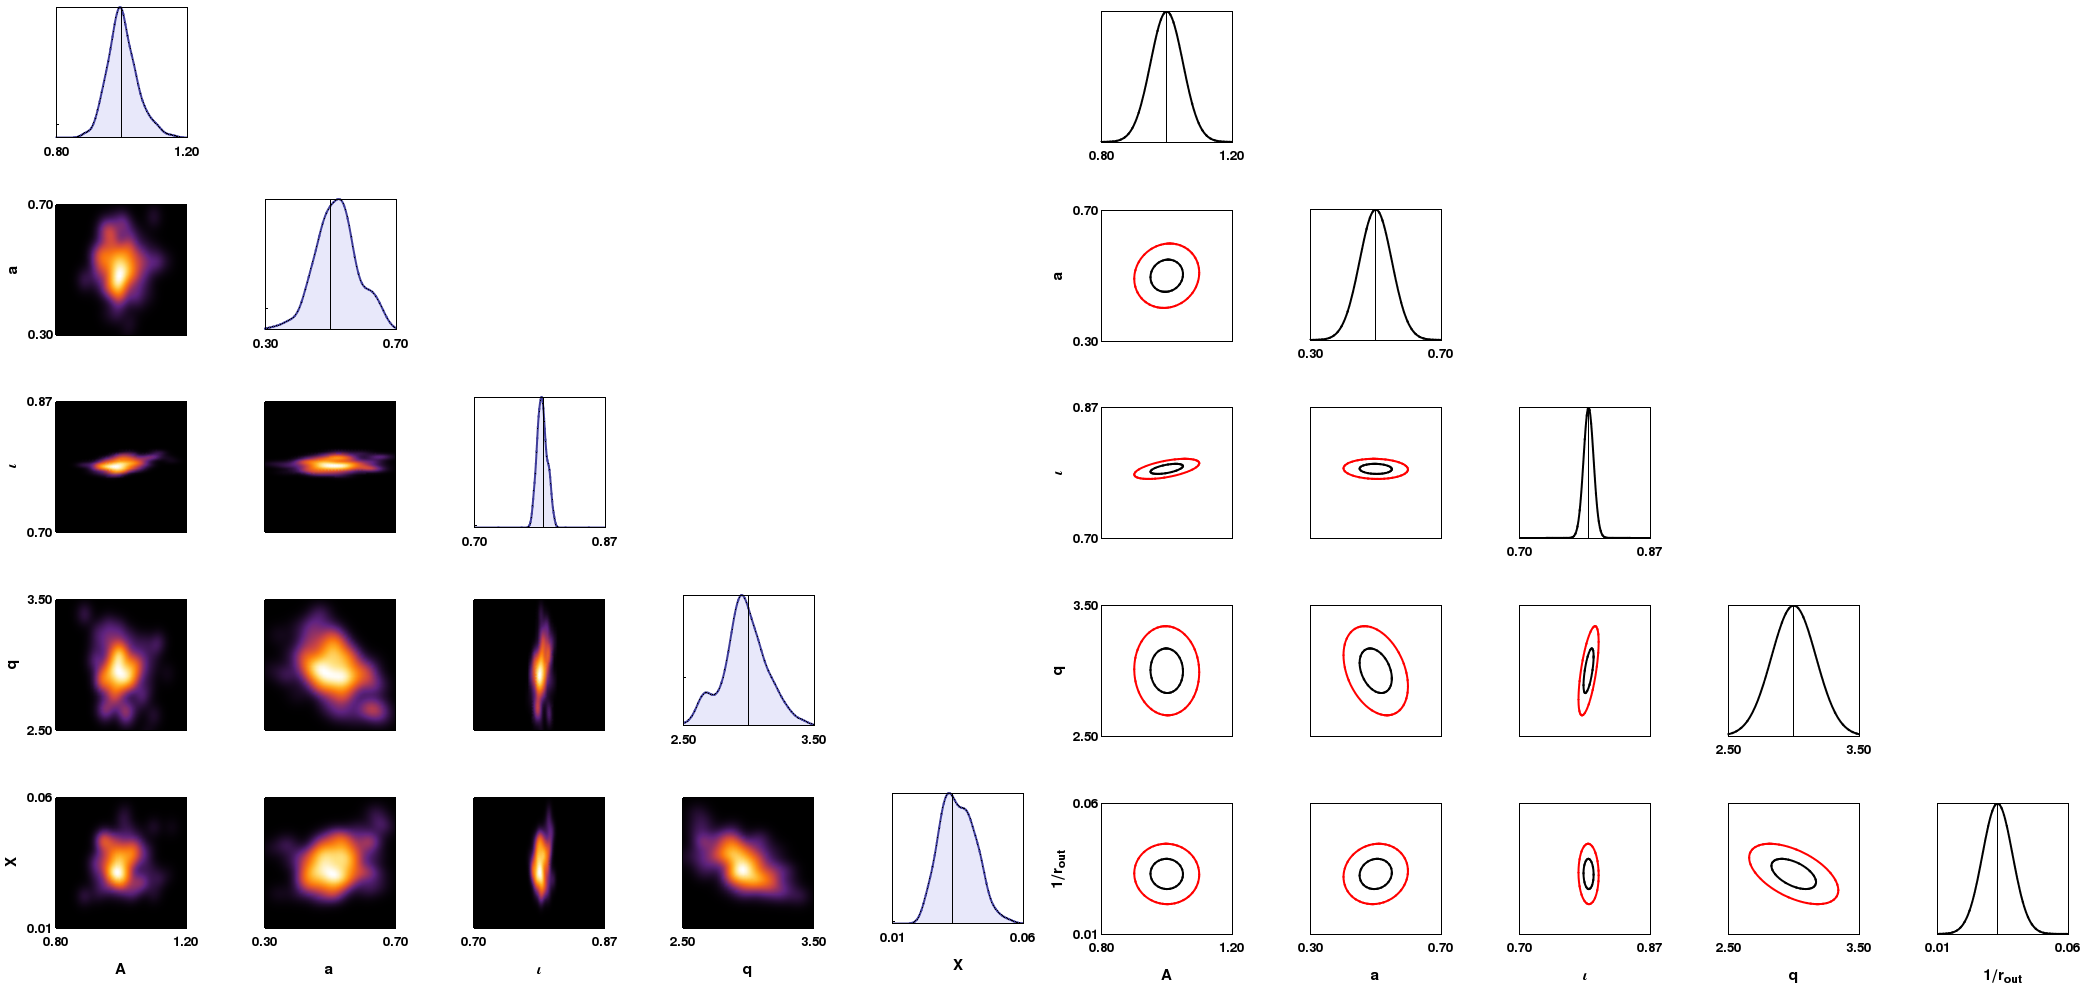
\includegraphics[trim=0cm 0cm 0cm 0cm, width=0.98\textwidth]{FishMCMC.png}
 \caption{A comparison of the likelihood surface predicted by the Fisher matrix (indicated by $1\sigma$ (black) and $2\sigma$ (red) contours) and the true posterior (shown as a density plot using samples produced from an MCMC algorithm). All parameters were set to their fiducial values; $A=1$, $a=0.5$, $\iota=\pi/4$, $q=3$ and $r_{\textrm{out}}=30$.}
 \label{fig:FishMCMC}
\end{figure*}

In order to calculate the likelihood it is first necessary to make some assumptions about the performance of our detector. For simplicity we assume that across the entire energy (frequency) range the detector has a constant energy (frequency) resolution $\Delta E$ ($\Delta f$),  and that in each energy (frequency) bin there is an independent Gaussian error of size $\sigma$. The values of $\Delta E = 100\,\textrm{eV}$ ($\Delta f=2.4\times 10^{14}\,\textrm{Hz}$) and $\sigma=0.05$ were choosen to make the hypothetical instrument broadly equivalent to the best current observations. For example, the error on the spin measurement for the fiducial disk parameters under these assumption is $\Delta a=0.06$ (see results in Fig.\ \ref{fig:FishMCMC}).

These simplifying assumptions neglect some important effects. For example, the frequency resolution of most X-ray detectors changes substantially across observable bandwidth, the random errors in each frequency bin are due to variations in the arrival rate of photons which is a Poisson not a Gaussian process (although in the limit of high signal-to-noise the assumption of Gaussian errors becomes correct), and in addition to the uncorrelated random errors there will be systematic errors which may be correlated between frequency bins. The effect of these simplifying assumptions is the following expression for the likelihood,
\begin{eqnarray}\label{eq:likelihood} 
&{\cal{L}}(\vec{\theta})&=\frac{\exp\left(\frac{-1}{2}\sum_{i=1}^{N}\frac{\left(s_{i}-h_{i}(\vec{\theta})\right)^{2}}{\sigma^{2}}\right)}{\sqrt{2\pi}\sigma^{N}} \nonumber \\
&&=\frac{\exp\left(\frac{-1}{2}\left<s-h(\vec{\theta})|s-h(\vec{\theta})\right>\right)}{\sqrt{2\pi}\sigma^{N}}\, ,\end{eqnarray}
where the inner product has been defined as
\begin{equation} \left<a|b\right>=\sum_{i=1}^{N}\frac{a_{i}b_{i}}{\sigma^{2}} \; . \end{equation}
In general Eq.\ \ref{eq:Bayes} is a complicated function of the parameters, $\vec{\theta}$. Expanding the signal about the true parameter values, $\vec{\theta_{0}}$, (using the Einstein summation convention)
\begin{equation}\label{eq:LSA} h(\vec{\theta})=h(\vec{\theta_{0}})+\frac{\partial h}{\partial\theta_{i}}  \Big|_{\vec{\theta}=\vec{\theta}_{0}}  \delta\theta_{i}+{\cal{O}}\left((\delta\theta_{i})^{2}\right)\;,\end{equation}
and using $s=n+h(\vec{\theta_{0}})$ (where $n$ is the particular realisation of the noise observed in the detector) gives
\begin{eqnarray}\label{eq:likelihood2} 
&{\cal{L}}(\vec{\theta})&\approx \frac{\exp\left(\frac{-1}{2}\left[(n|n)-2\left(n|\frac{\partial h}{\partial\theta_{i}}\big|_{\vec{\theta}=\vec{\theta}_{0}}\delta\theta_{i}\right)+\Sigma_{ij}\delta\theta_{i}\delta\theta_{j}\right]\right)}{\sqrt{2\pi}\sigma^{N}}\, ,\nonumber\\
&&\;\textrm{where}\; \Sigma_{ij}=\left<\left.\frac{\partial h(\vec{\theta})}{\partial \theta_{i}}\Big|_{\vec{\theta}=\vec{\theta}_{0}}\right|\frac{\partial h(\vec{\theta})}{\partial \theta_{j}}\Big|_{\vec{\theta}=\vec{\theta}_{0}}\right> \; .\end{eqnarray}
Therefore, within the linear signal approximation used in Eq.\ \ref{eq:LSA}, the likelihood is a multivariate Gaussian, peaked at the true parameters, and with a covariance matrix given by the inverse of the Fisher information matrix, $\Sigma_{ij}$. An estimate for the error in each parameter may be read off from the corresponding component of the covariance matrix,
\begin{equation} \Delta\theta_{i}=\sqrt{\left(\Sigma^{-1}\right)_{ii}} \quad\textrm{(no sum on $i$).} \end{equation}
The Fisher matrix formalism was used first for the Kerr metric (Sec.\ \ref{subsubsec:kerrres} below) and subsequently for all of the bumpy black hole spacetimes discussed in Sec.\ \ref{sec:spacetimes} (Secs.\ \ref{subsubsec:KSres} to \ref{subsubsec:B2res} below). In the case of the bumpy black hole spacetimes the true value of the bump parameter was set to zero, i.e.\ the Kerr metric was used, and the error estimate obtained for the bump is reported. The error on the bump parameter(s) are then interpreted as an estimate of the bound it may be possible to place on the size of the bump; i.e.\ if the true value of the bump parameter took this value then it would be marginally detectable with these observations. This bound should be interpreted as a lower limit, i.e.\ a best case scenario; in reality even if a non-zero value of a given deformation parameter was returned in a particular experiment it would still be a non-trivial task to rule out more mundane explanations. For example, before claiming a detection of a deviation from the Kerr solution it would presumably be necessary to consider more complicated forms for the radial emissivity, $\epsilon(r)$, than a simple power law. The free parameters in this new emissivity law would then have to be marginalised over and this would have the effect of increasing the errors on the other parameters. Other possibilities must also be considered; for example thick accretion disks, emitting material within the ISCO, reprocessing of the light by surrounding material, etc.

The applicability of the Fisher matrix rests on the validity of the linear signal approximation in Eq.\ \ref{eq:LSA}; this must hold at least within a few standard deviations from the peak in all directions in parameter space. In general it is impossible to know from the Fisher matrix alone whether one is within the region where the linear signal approximation may be safely applied. This question of the applicability of the Fisher matrix is addressed in Sec.\ \ref{subsec:validityFish}.

\section{Verification of the applicability of the Fisher matrix formalism}\label{subsec:validityFish}
The gold standard for parameter estimation is to numerically calculate the likelihood (or in general the posterior) surface over the region of parameter space of interest. This may be achieved in low dimensional problems by simply evaluating the likelihood function on a grid of parameter points. Alternatively, and more efficiently in high dimensional problems, there exist a variety of Markov chain Monte Carlo (MCMC) algorithms designed to sample points from the target probability distribution; the simplest of these is the Metropolis-Hastings algorithm. In Secs.\ \ref{subsubsec:MCMC} a MCMC analysis is performed on a sample Iron line spectra for a typical case; the resulting likelihood surfaces are compared with those predicted using the Fisher matrix.

\begin{figure*}[t]
 \centering
 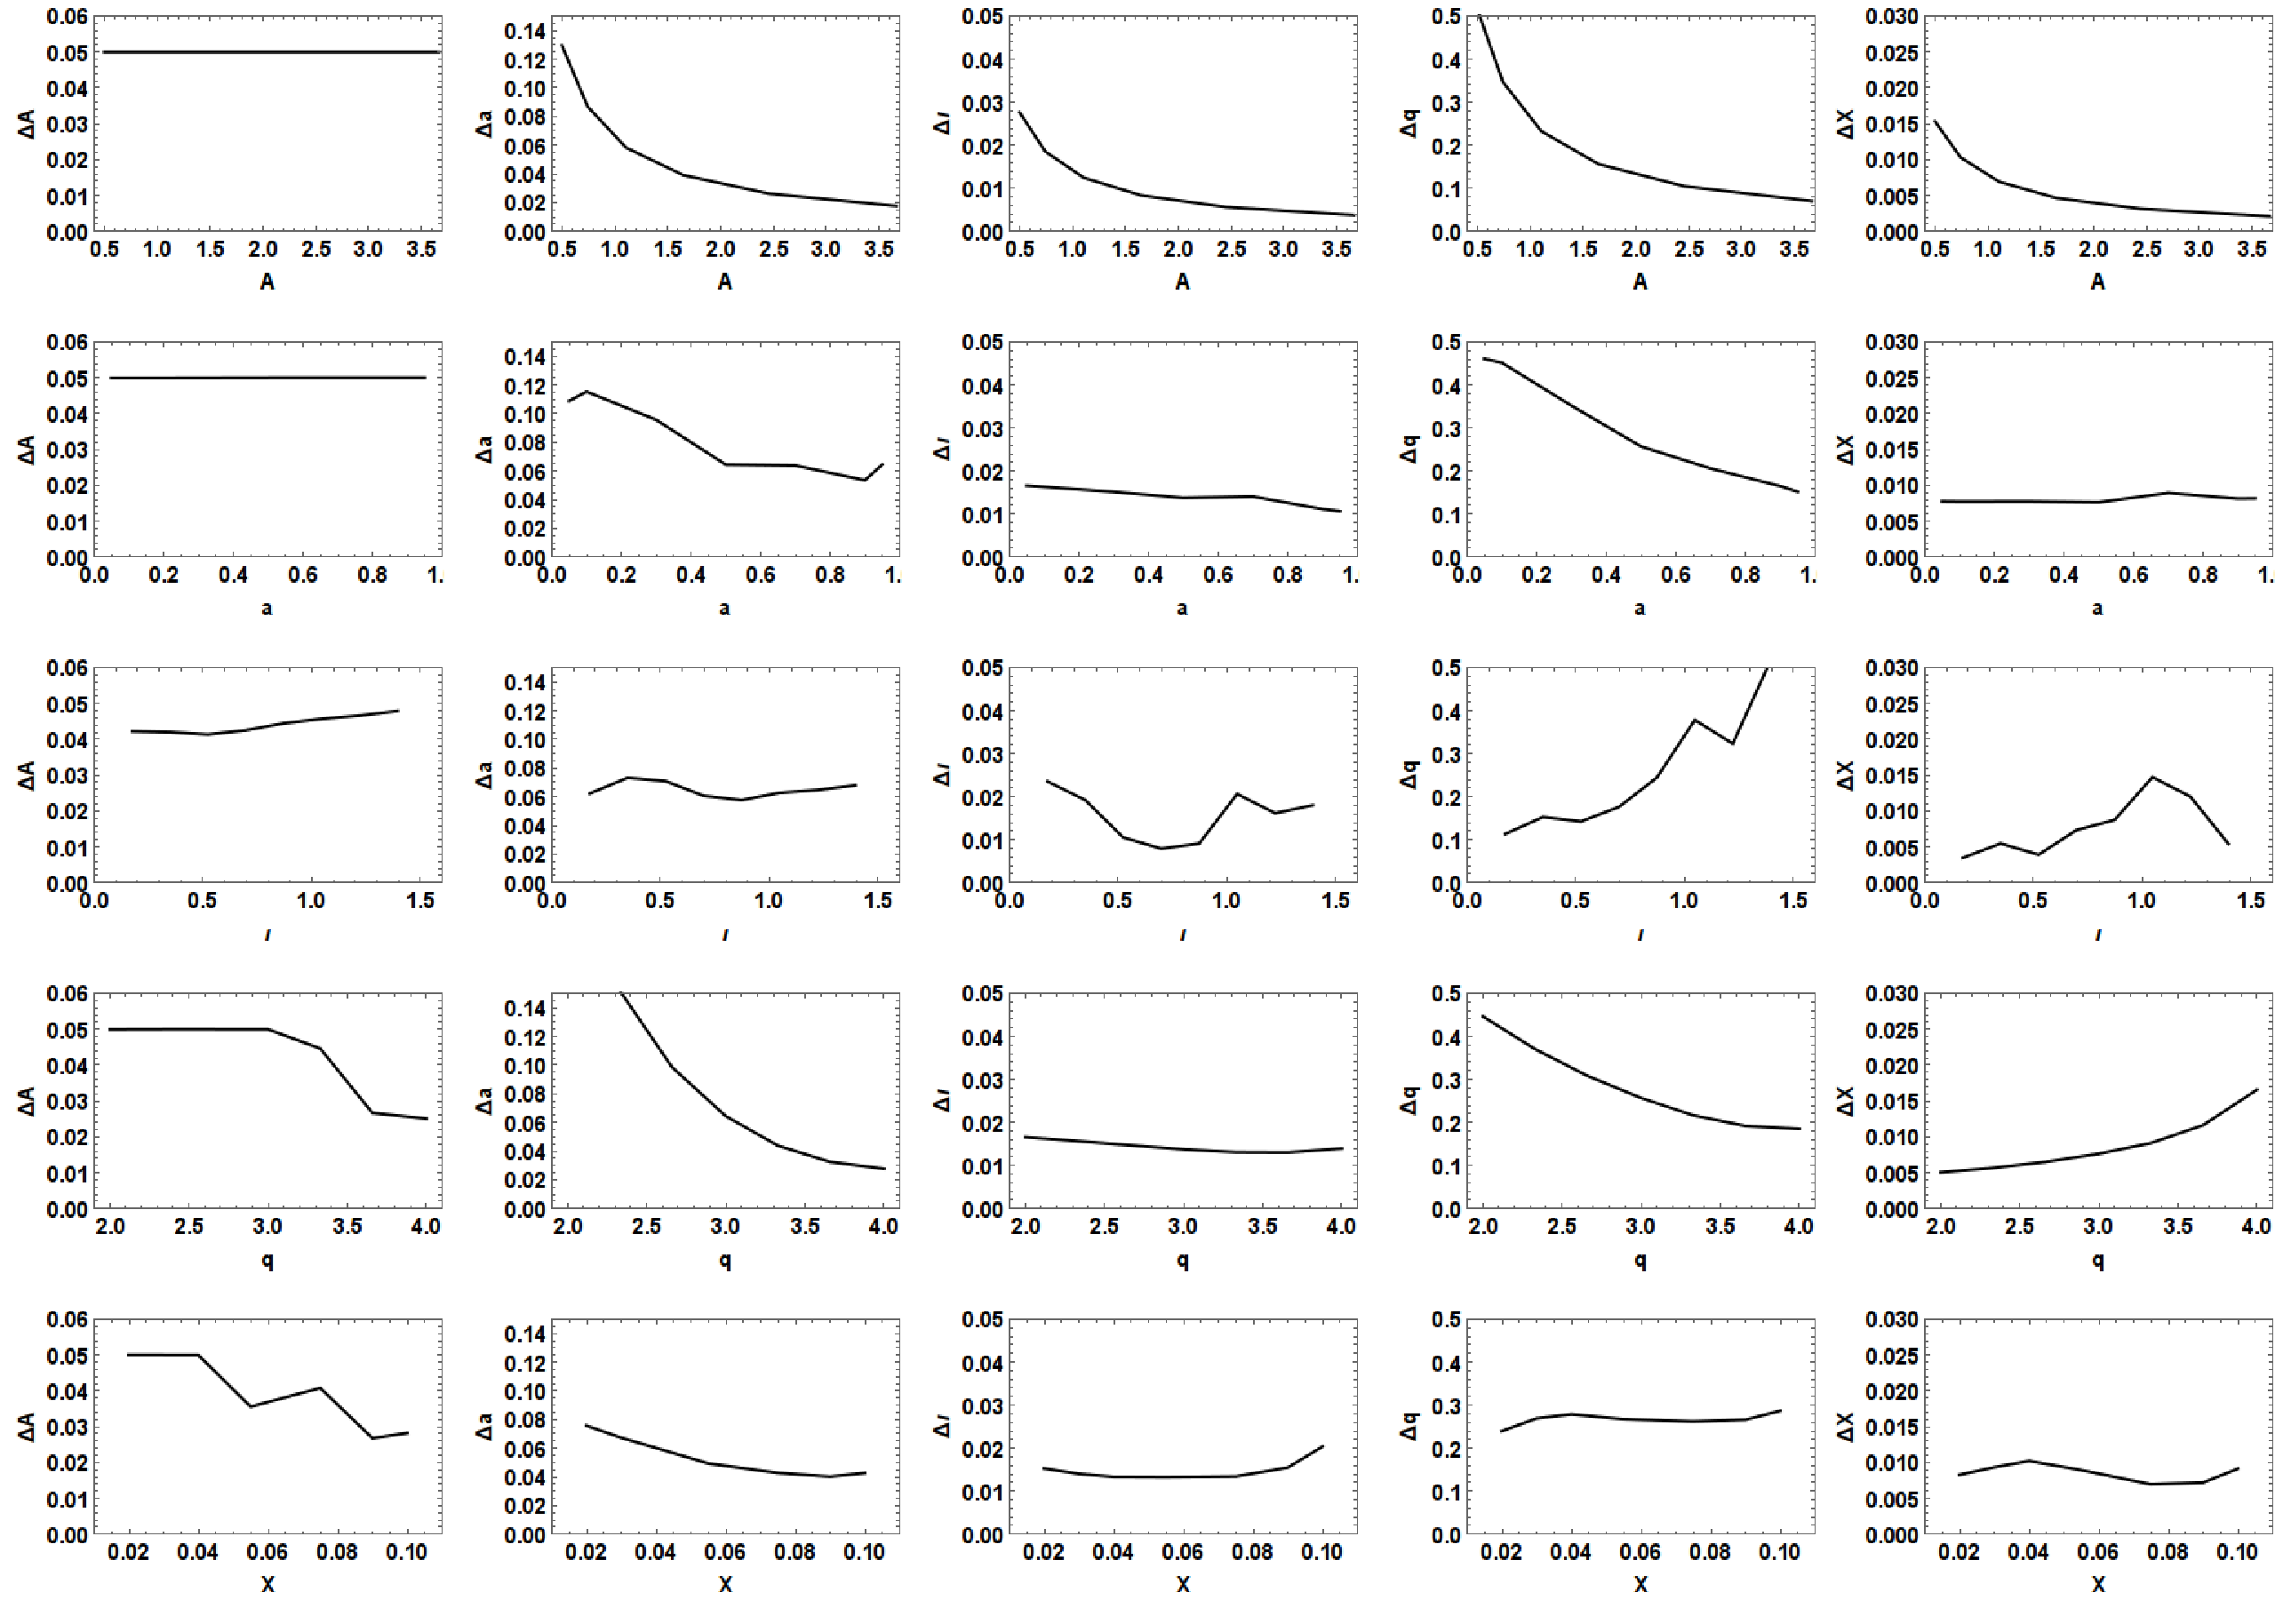
\includegraphics[trim=0cm 0cm 0cm 0cm, width=0.95\textwidth]{KerrFisherMatrixErrors2.pdf}
 \caption{Each panel of this figure gives the error in the column parameter versus the value of the row parameter for fixed fiducial values of the other parameters; $A=1$, $a=1$, $\iota=\pi/4$, $q=3$ and $r_{\textrm{out}}=30$.}
 \label{fig:KerrFisherMatrixErrors}
\end{figure*}

MCMC type algorithms quickly become (prohibitivly) expensive as the dimension of the parameter space increases. \cite{Vallisneri} proposed a consistancy check on the Fisher matrix which is relativly quick to implement. The consistancy check involves testing the validity of the linear signal approximation. For some central parameter values, $\vec{\theta_{0}}$, a point $\vec{\theta}$ is picked at random from the $1\sigma$ surface estimated by the Fisher matrix. The likelihood is then evaluated exactly, and approximated with the linear signal approximation, the ratio of the two likelihoods is denoted $r(\vec{\theta})$. The logarithm of this ratio is given by
\begin{eqnarray}\label{eq:val} 
&&\left| \log   r(\vec{\theta}) \right| =\frac{1}{2}\left.\left(\Delta\theta_{i}h_{i}-\Delta h(\vec{\theta})\right\vert\Delta\theta_{i}h_{i}-\Delta h(\vec{\theta})\right) \, ,\nonumber\\
&&\quad\quad\textrm{where }\Delta\vec{\theta}=\vec{\theta}-\vec{\theta}_{0}\,,\; \Delta h (\vec{\theta})=h(\vec{\theta})-h(\vec{\theta}_{0})\,,\nonumber \\
&&\quad\quad\textrm{and }\, h_{i}=\left.\frac{\partial h(\vec{\theta})}{\partial \theta^{i}}\right|_{\vec{\theta}=\vec{\theta}_{0}} .\end{eqnarray}
Small values of $|\log r(\vec{\theta})|$ incate that the linear signal approximation is holding out as far as the $1\sigma$ surface in that particular parameter direction. This procedure may then be repeated for many points drawn randomly from the $1\sigma$ surface to assess whether the approximation holds in all directions. It should be stressed that this only checks the internal consistency of the linear signal approximation and does not guarantee the accuracy of the Fisher matrix. In Sec.\ \ref{subsubsec:val} this consistency check was performed for the Iron line emission likelihood surface, as the consistency check is faster than a full MCMC it was performed for a range of spin and inclination parameter values.

\subsection{MCMC}\label{subsubsec:MCMC}
A simple Metropolis-Hastings MCMC was used to sample from the likelihood distribution in Eq.\ \ref{eq:likelihood} with the Iron line spectra described in Sec.\ \ref{subsec:line}. The resulting chain, plotted as a density histogram, is shown in Fig.\ \ref{fig:FishMCMC} alongside the Gaussian contours from the Fisher matrix analysis. From Fig.\ \ref{fig:FishMCMC} it can be seen that there is unquestionably additional structure in the true posterior which is not captured by the Fisher matrix; however the widths of the Fisher matrix Gaussians give a good indiction of the scale of the true posterior.

\begin{table}[h]
\begin{center}
\begin{tabular}{ l | c c c c }
	&$\iota=\frac{\pi}{10}$&$\iota=\frac{2\pi}{10}$&$\iota=\frac{3\pi}{10}$&$\iota=\frac{4\pi}{10}$\\
\hline
$a=0.1$ & 0.0044/0.013	& 0.0088/0.032	& 0.025/0.15	& 0.10/0.50	\\
$a=0.3$ & 0.0046/0.016	& 0.0091/0.030	& 0.022/0.064	& 0.032/0.14	\\
$a=0.5$ & 0.0037/0.0069	& 0.011/0.026	& 0.019/0.083	& 0.028/0.077	\\
$a=0.7$ & 0.0039/0.0095	& 0.012/0.036	& 0.017/0.061	& 0.028/0.088	\\
$a=0.9$ & 0.0078/0.015	& 0.014/0.028	& 0.027/0.053	& 0.031/0.10	\\
\end{tabular}
\end{center}
\caption{All entries are of the form $\mu$/$M$, where $\mu$ is the mean value of the logarithm of mismatch ratio calculated on 100 points selected uniformly from the $1\sigma$ surface and $M$ is the maximum value of the mismatch ratio on the same set of points. All other parameters were set to their fiducial values of $A=1$, $q=3$ and $r_{\textrm{out}}=30$. (The forward slash between entries does \emph{not} indicate division.)}
\label{tab:val}
\end{table}


\subsection{Mismatch ratio}\label{subsubsec:val}
For a range of values of $a$ and $\iota$ the Fisher matrix was evaluated, and used to choose $100$ points, randomly distributed, on the $1\sigma$ surface. The mismatch ratio was evaluated for all of these points and the results are summarised in Tab.\ \ref{tab:val}; all values are less that unity, indicating that the Fisher matrix could be applicable to this problem.

\section{Results}\label{sec:results}
\subsection{Kerr errors: Iron line}\label{subsubsec:kerrres}
The Fisher matrix formalism was used to assess the accuracy with which it might be possible to measure the parameters $\left\{A,a,\iota,q,X\right\}$ with the Iron line observations described in Sec.\ \ref{subsec:line}. The results are shown in Fig.\ \ref{fig:KerrFisherMatrixErrors}.


\begin{figure*}[t]
 \centering
 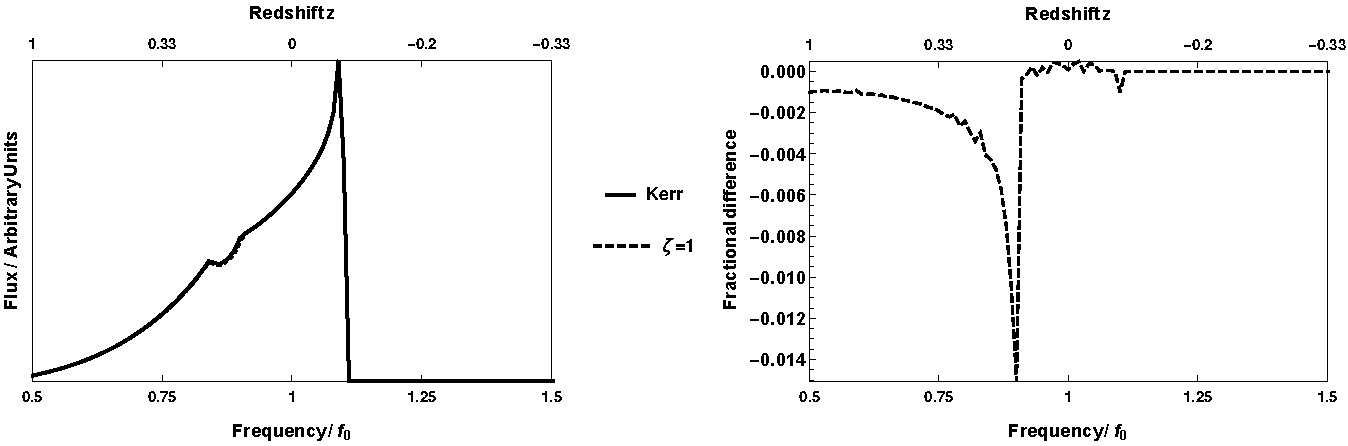
\includegraphics[trim=0cm 0cm 0cm 0cm, width=0.9\textwidth]{CS2IronLines.pdf}
 \caption{The left-hand panel shows a pair of Iron line spectra for accretion disks around a Kerr black hole and a quadratic in spin CS black hole (CS2 metric) with a large deformation, $\zeta=1$. Also shown in the right-hand panel is the residual plot. All parameters were set to their fiducial values; $A=1$, $a=0.5$, $\iota=\pi/4$, $q=3$ and $r_{\textrm{out}}=30$.}
 \label{fig:CS1IronLines}
\end{figure*}

\subsection{KS metric}\label{subsubsec:KSres}
The formalism described in Sec.\ \ref{sec:emission} was used to calculate the Iron line profile in the KS metric, Eq.\ \ref{eq:KSmetric}. As described in Sec.\ \ref{sec:emission} the shift in the position of the ISCO, relative to the Kerr values, to first order in the small parameter $1/\omega$ may be calculated; $r_{isco}=r_{isco}^{\textrm{Kerr}}+\Delta r_{isco}$, where 
\begin{equation} \Delta r_{isco}=\frac{-11}{36\omega}-\frac{59a}{54\sqrt{6}\omega}\, .  \end{equation}
The ISCO moves inwards for increasing deformation, therefore the effect of a large value of $1/\omega$ is to boost the redshifted red wing of the line profile relative to the blue-shifted peak, similar to the effect of increasing spin; see Fig.\ \ref{fig:KSIronLines}. 

\begin{figure}[h]
 \centering
 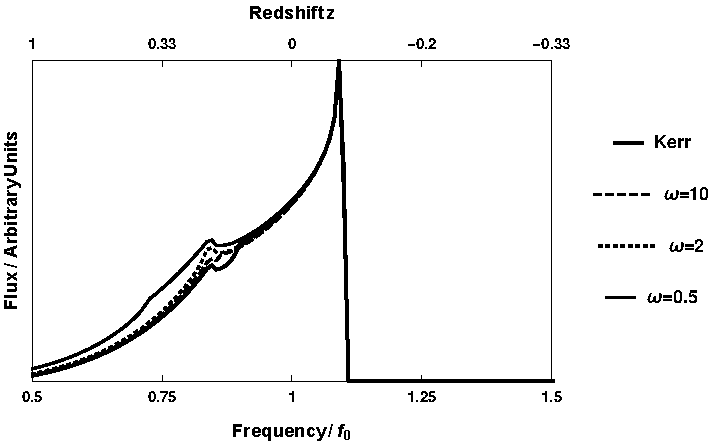
\includegraphics[trim=0cm 0cm 0cm 0cm, width=0.45\textwidth]{KSIronLines.pdf}
 \caption{A series of Iron line spectra for accretion disks around KS black holes varying the value of $\omega$. All other parameters were set to fiducial values, $a=0.5$, $\iota=\pi/4$, $q=3$ and $r_{\textrm{out}}=30$.}
 \label{fig:KSIronLines}
\end{figure}

The $1\sigma$ and $2\sigma$ contours from a Fisher matrix analysis are plotted in Fig.\ \ref{fig:KSFish}, it can be seen that there is a rather stark degeneracy between the spin and deformation parameter. By comparing Fig.\ \ref{fig:KSFish} to Fig.\ \ref{fig:FishMCMC} it can be seen that the errors in all other parameters are virtually unaffected by the inclusion of the deformation parameter. The effect of the degeneracy, apart from inhibiting any measurement of the spin parameter, is to make it very difficult to place any bound on the deformation; Tab.\ \ref{tab:KS} gives the bound it is possible to place on $\omega$ for different values of spin. It should be remembered that the KS metric is valid only to linear order in $a$, and in addition the metric exhibits unphysical properties (e.g. naked singularities, closed timelike curves, etc) for $\omega < 1/2$. Therefore, bearing in mind the fact that the bounds derived from the method discussed in Sec.\ \ref{sec:analysis} should be treated as lower limits, the conclusion to be drawn from Tab.\ \ref{tab:KS} is that no meaningful bound can be placed on the KS deformation parameter using observations of the Iron K$\alpha$ line profile.

\begin{figure*}[t]
 \centering
 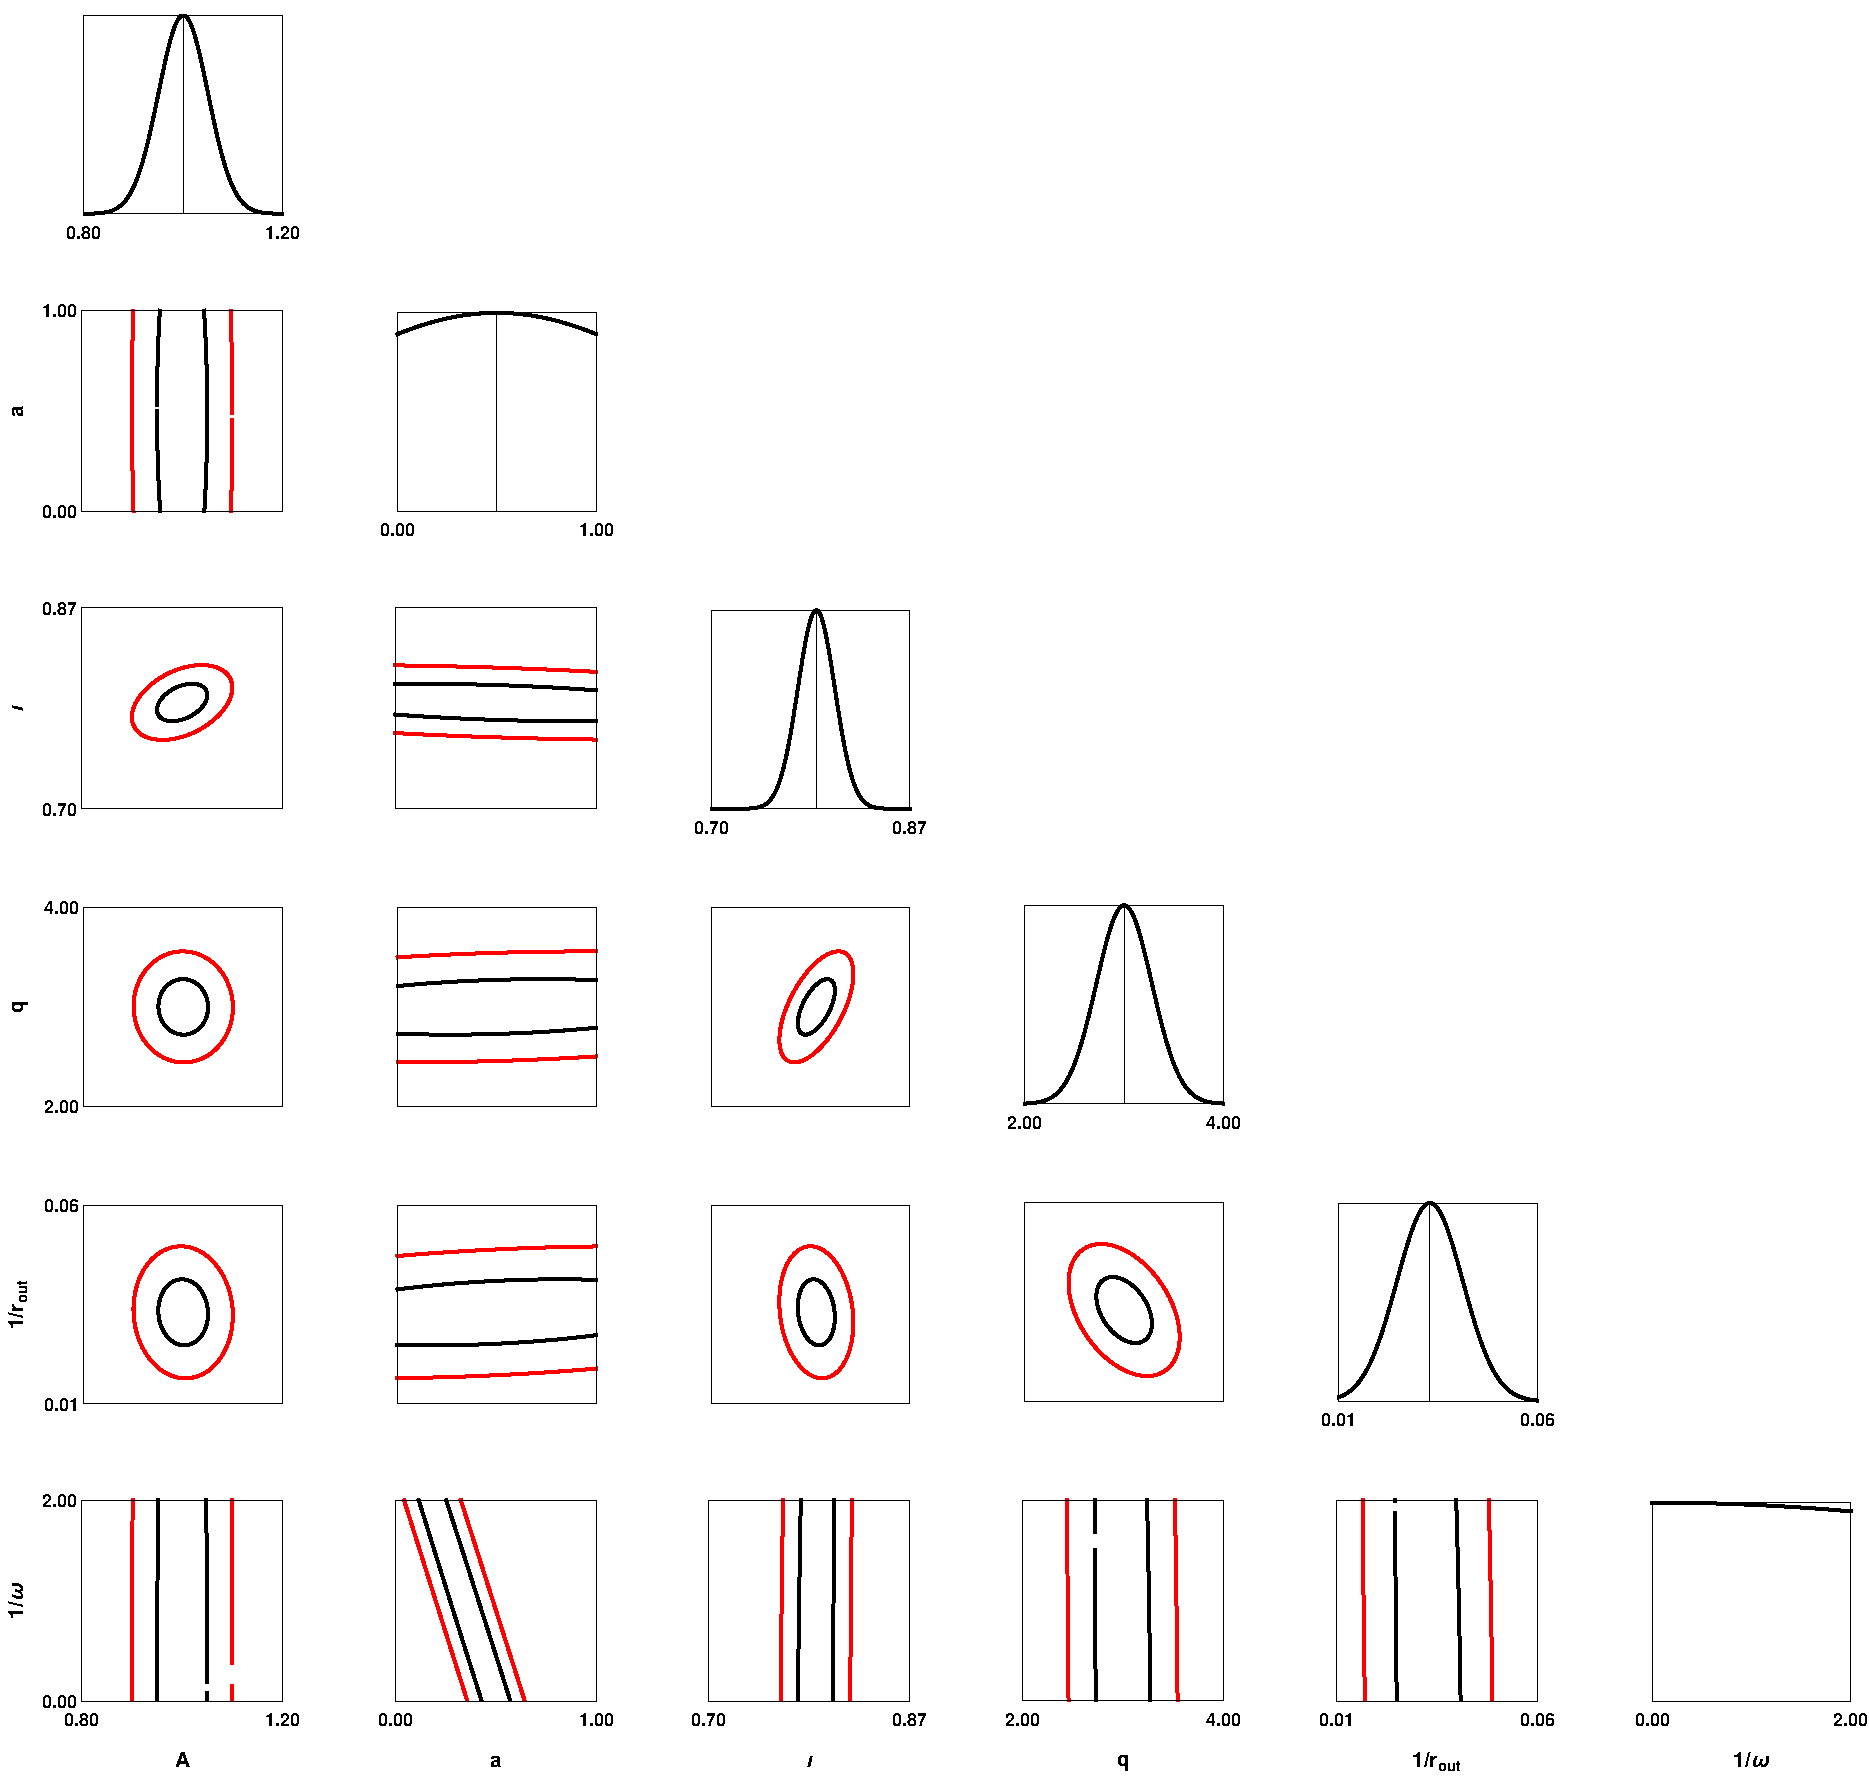
\includegraphics[trim=0cm 0cm 0cm 0cm, width=0.85\textwidth]{KSFisherPlot.pdf}
 \caption{The $1\sigma$ and $2\sigma$ contours from a Fisher matrix analysis on the KS metric. It can be seen that introducing the extra degree of freedom in the KS deformation parameter has introduced a clear degeneracy with the spin parameter. From the bottom righthand plot it can be seen that the data is almost equally consistent with any value of $\omega$ in the range $(1/2,\infty)$, so no bound may be placed in the deformation. All parameters were set to their fiducial values; $A=1$, $a=0.5$, $\iota=\pi/4$, $q=3$, $r_{\textrm{out}}=30$ and $Y\equiv 1/\omega=0$.}
 \label{fig:KSFish}
\end{figure*}

There have been several attempts to place bounds on the KS deformation parameter using solar system tests of gravity such as perihelion precession, deflection of light by the Sun and radar echo delay observations \citep{2011GReGr..43.1401L,2011RSPSA.467.1390H,2011IJMPD..20.1079I}. The bounds obtained from these studies are typically on the length scale $\omega\gtrsim 5\times 10^{-28}\,\textrm{m}$, corresponding to a dimensionless bound $\omega M^{2} \gtrsim 3\times 10^{-16}$, with $M=\Msun$. It should be noted that these bounds are much less stringent than the requirement imposed here that $\omega>1/2$, which is necessary to ensure that there is an event horizon. However, as these tests were conducted in the weak field around a material object whose radius is much larger than the gravitational radius the vacuum solution is not valid down near the event horizon and the constriant $\omega>1/2$ need not apply.

\begin{table}[h]
\begin{center}
\begin{tabular}{ l | c  }
	&$\Delta (1/\omega)$\\
\hline
$a=0.1$ &  15.2 \\
$a=0.3$ &  9.23 \\
$a=0.5$ &  5.47 \\
$a=0.7$ &  4.76 \\
$a=0.9$ &  3.44 \\
\end{tabular}
\end{center}
\caption{The Bounds it is possible to place on the small KS deformation parameter ($1/\omega$) for different values of the spin parameter, $a$. All other parameters were set to their fiducial values; $A=1$, $\iota=\pi/4$, $q=3$ and $r_{\textrm{out}}=30$ and $Y\equiv 1/\omega=0$.}
\label{tab:KS}
\end{table}



\subsection{CS metric}\label{subsubsec:CS1res}
Shown in Fig.\ \ref{fig:CS1IronLines} is the Iron line profile for a Kerr black hole and a CS2 black hole with deformation $\zeta=1$. It should be remembered that the CS1 and CS2 metrics in Eqs.\ \ref{eq:CS1metric} and \ref{subsec:CS2} are only valid in the limit $\zeta\ll 1$. However, even with the large deformation used in Fig.\ \ref{fig:CS1IronLines} the change in the line profile is only visible in the residual plot shown in the right-hand panel. The Iron line profile for the CS1 metric shows very similar behaviour to that in Fig.\ \ref{fig:CS1IronLines}.

Bearing in mind the results in Fig.\ \ref{fig:CS1IronLines}, it is clear that it will be extremely difficult to bound the CS1 deformation parameter using this technique. Tab.\ \ref{tab:CS1} shows the bounds it is possible to place on both the CS1 and CS2 deformation parameters for a range of values of $a$; it was found that no bounds less than unity were possible with Iron line observations, however, the best results were obtained for the CS1 metric and high values of spin. Both the CS1 and CS2 metrics are expansions in the $a$ parameter, therefore the bounds for the higher values of spin (particularly $a=0.9$) should be treated with more caution than the low spins. However, this does not effect our main conclusion that no bounds less than unity were possible. 

For comparison, weak field tests using the frame-dragging effect around the Earth measured by the Gravity Probe B and the LAGEOS satellites places a bound $\zeta^{1/4}<10^{8}\,\textrm{km}$ \citep{2011PhRvD..84l4033A} corresponding to a dimensionless bound of $\zeta < 2\times 10^{14}$. Tighter bounds will be possible using strong field tests, for example it was found that bounds of $\zeta^{1/4}<10^{4}\,\textrm{km}$ corresponding to a dimensionless bound of $\zeta < 2\times 10^{14}$ would be possible with eLISA observations of EMRIs \citep{2012PhRvD..86d4010C}.

\begin{table}[h]
\begin{center}
\begin{tabular}{ l | c  c }
	&$\Delta \zeta_{\textrm{CS1}}$ &$\Delta\zeta_{\textrm{CS2}}$\\
\hline
$a=0.1$ & 101  & 122	\\
$a=0.3$ & 97.0 & 62.6	\\
$a=0.5$ & 24.0 & 25.4	\\
$a=0.7$ & 23.9 & 9.98	\\
$a=0.9$ & 1.32 & 5.34	\\
\end{tabular}
\end{center}
\caption{The Bounds it is possible to place on the CS1 and CS2 deformation parameters for different values of the spin parameter, $a$. It should be remembered that the CS parameter is constrained to be $\zeta\ll 1$, therefore no meaningful constraint may be placed with these observations. All other parameters were set to fiducial values, $A=1$, $\iota=\pi/4$, $q=3$, $r_{\textrm{out}}=30$ and $\zeta=0$.}
\label{tab:CS1}
\end{table}

\subsection{${\cal{B}}_{N}$ metrics}\label{subsubsec:B2res}
Shown in Fig.\ \ref{fig:B2Line} are a series of Iron line profiles for the metrics defined in Sec.\ \ref{sec:spacetimes} with the constants ${\cal{B}}_{2}$ varied. The deformation parameters were varied between 0 and 0.5. Shown in Tab.\ \ref{tab:B2} is the bounds it is possible to place on the different deformations using Iron line observations for different values of $a$.
\begin{figure*}[t]
 \centering
 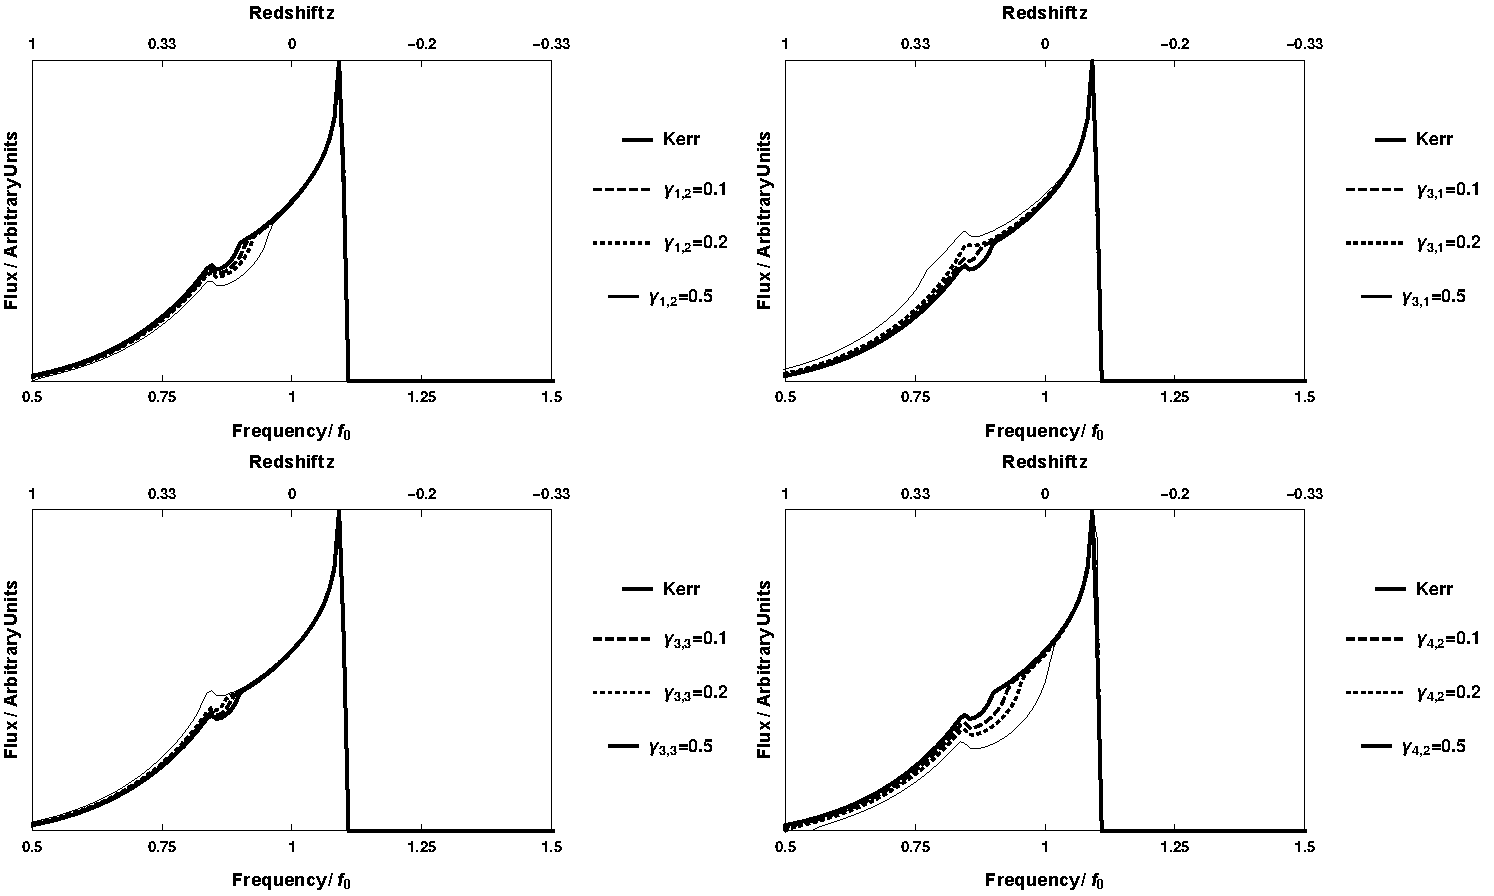
\includegraphics[trim=0cm 0cm 0cm 0cm, width=0.9\textwidth]{B2IronLines.pdf}
 \caption{A series of Iron line spectra for accretion disks around B2 bumpy black holes with varying values of the bump parameters. All other parameters were set to fiducial values; $A=1$, $a=0.5$, $\iota=\pi/4$, $q=3$, $r_{\textrm{out}}=30$, and $\gamma_{i,j}=0$ unless otherwise indicated.}
 \label{fig:B2Line}
\end{figure*}

The results in Tab.\ \ref{tab:B2} show that the tightest constraints on the ${\cal{B}}_{N}$ bumpy black holes can be placed on the lowest values of $N$ for the highest values of spin. The lower values of $N$ have deformations entering at lower powers of $1/r$, since all the emission originates from outside the horizon (where $r>1$) it is to be expected that deformations at lower $N$ are easier to constrain. It is also to be expected that higher values of spin make placing constraints easier, because the ISCO moves to smaller values of $r$ for larger spins, and most of the emission comes from close to the ISCO, the deformation has a greater effect on the spectra for high spins. These trends are summarised in Fig.\ \ref{fig:summary} where the tightest bound for each ${\cal{B}}_{N}$ is plotted as a function of spin.

\begin{table*}[t]
\resizebox{1.0\textwidth}{!}{\begin{minipage}{\textwidth}
\begin{center}
\begin{tabular}{ l | c c c c | c c c | c c c | c c c }
	& \multicolumn{4}{ |c| }{${\cal{B}}_{2}$} &\multicolumn{3}{ |c }{${\cal{B}}_{3}$} 	& \multicolumn{3}{ |c| }{${\cal{B}}_{4}$} &\multicolumn{3}{ |c }{${\cal{B}}_{5}$} \\
	&$\Delta\gamma_{1,2}$&$\Delta\gamma_{3,1}$ & $\Delta\gamma_{3,3}$&$\Delta\gamma_{4,2}$ 	&$\Delta\gamma_{1,3}$&$\Delta\gamma_{3,4}$&$\Delta\gamma_{4,3}$ 	&$\Delta\gamma_{1,4}$&$\Delta\gamma_{3,5}$&$\Delta\gamma_{4,4}$	&$ \gamma_{1,5}$&$\Delta\gamma_{4,5}$&$\Delta\gamma_{3,6}$\\
\hline
$a=0.1$ & 3.1  & 15    & 6.0  & 1.7  	& 64   & 20   & 33 	& 120 & 41   & 70 	& 180 & 47   & 160  \\
$a=0.3$ & 0.93 & 4.5   & 5.8  & 0.38 	& 55   & 5.1  & 27 	& 54  & 35   & 29 	& 80  & 19   & 120  \\
$a=0.5$ & 0.67 & 1.3   & 6.1  & 0.25 	& 41   & 1.4  & 18 	& 50  & 18   & 25 	& 27  & 3.7  & 78   \\
$a=0.7$ & 0.33 & 0.15  & 0.42 & 0.17 	& 3.6  & 0.50 & 1.5 	& 29  & 7.8  & 12 	& 8.2 & 2.6  & 12   \\
$a=0.9$ & 0.36 & 0.025 & 0.20 & 0.11 	& 0.81 & 0.24 & 0.32 	& 4.1 & 0.72 & 1.6	& 1.0 & 0.50 & 1.6  \\
\end{tabular}
\end{center}
\caption{The Bounds it is possible to place on the different ${\cal{B}}_{N}$ bump parameters for different values of the spin parameter, $a$. The tightest bounds can typically be placed for low values of $N$ (i.e.\ ${\cal{B}}_{2}$) and for the most highly spinning black holes. All other parameters were set to fiducial values; $A=1$, $\iota=\pi/4$, $q=3$, $r_{\textrm{out}}=30$ and $\epsilon =0$. }
\label{tab:B2}
\end{minipage} }\end{table*}

\begin{figure*}[t]
 \centering
 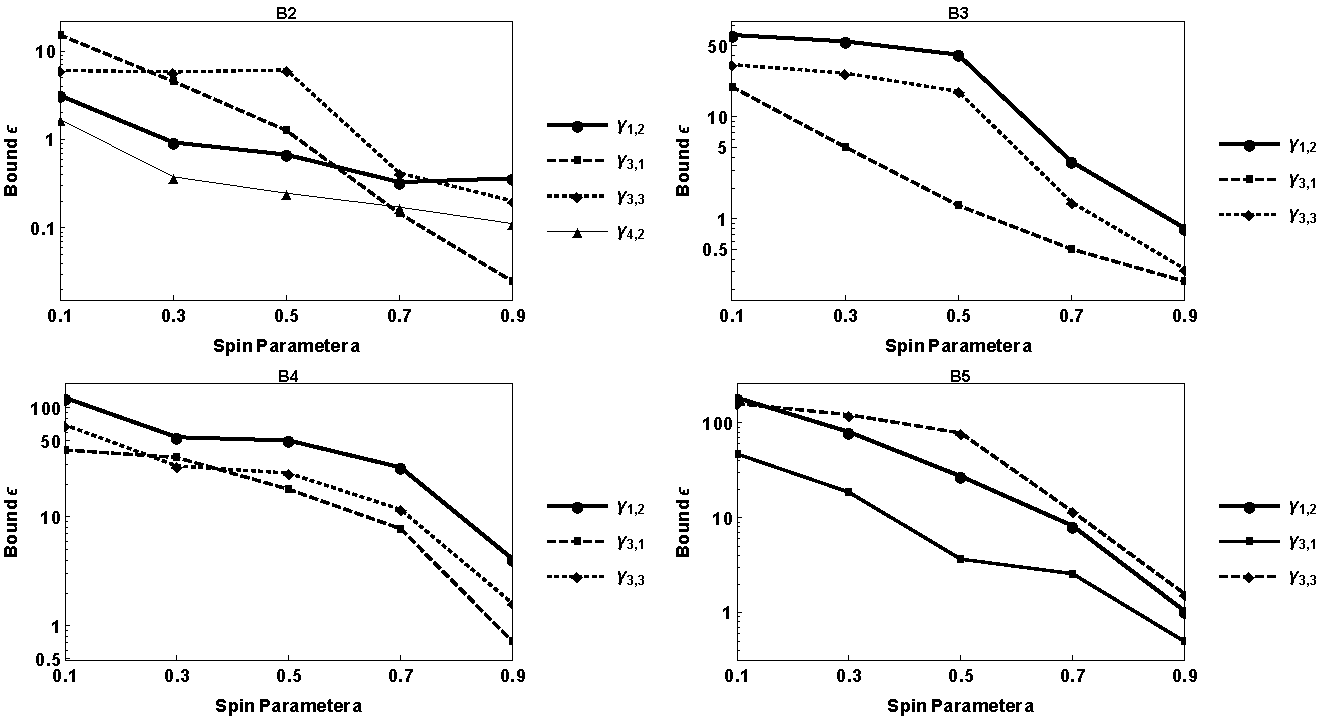
\includegraphics[trim=0cm 0cm 0cm 0cm, width=0.9\textwidth]{fig_summary.pdf}
 \caption{The bounds on the ${\cal{B}}_{N}$ parameters from Tab.\ \ref{tab:B2} plotted as a function of the spin parameter. It can be seen that the tightest bound may be placed for the ${\cal{B}}_{2}$ deformation around a highly spinning black hole.}
 \label{fig:summary}
\end{figure*}



